\section{Notation}
\begin{itemize}
    \item $X \sim N(\mu,\sigma^2)$
    \item $\mu$ = mean of the population
    \item $\sigma^2$ = \textbf{variance} of the data
\end{itemize}
\section{Properties}
\begin{itemize}
    \item The data is \textbf{continuous}
    \item Has parameters $\mu$ (mean) and $\sigma^2$ (variance)
    \item Is symmetrical: mean = median = mode
    \item Has a bell-shaped curve with asymptotes at each end
    \item Total area under the curve = $1$
    \item Has points of inflection at $\mu+\sigma$ and $\mu-\sigma$
\end{itemize}

\section{Estimating probabilities}
\begin{itemize}
    \item $68\%$ of observations lie within $\pm 1$ standard deviation of the mean
    \item $95\%$ of observations lie within $\pm 2$ standard deviation of the mean
    \item $99.8\%$ of observations lie within $\pm 3$ standard deviation of the mean
\end{itemize}
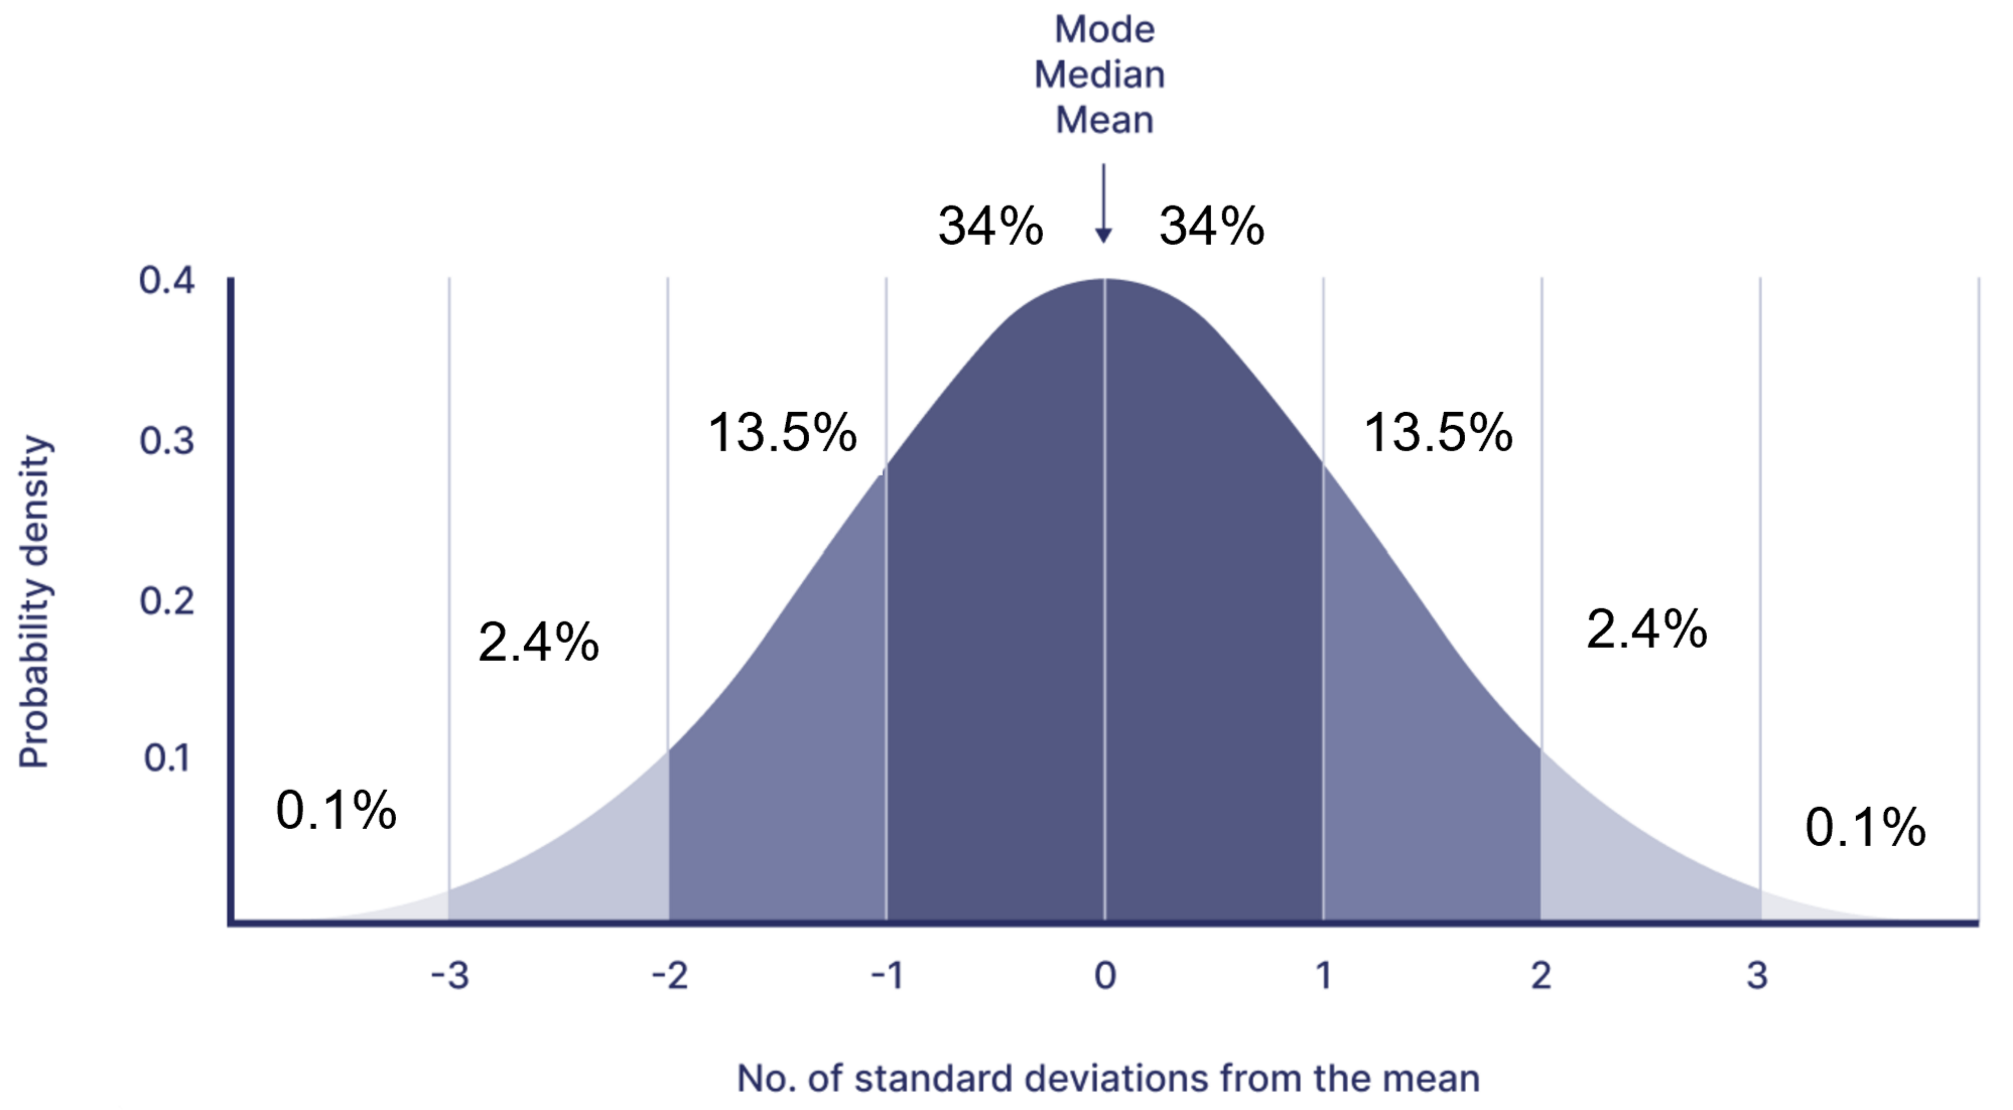
\includegraphics[width=0.7\linewidth]{images/normal_estimate}

\section{Approximation of binomial distribution}
If $n$ is large ($n\geq35$) and $p$ is close to $0.5$, then $X \sim B(n,p)$ can be modelled as $$Y \sim N(np, np(1-p))$$
\subsection{Approximations}
\begin{itemize}
    \item $\text{P}(X\geq a)\approx \text{P}(Y\geq [a-0.5])$
    \item $\text{P}(X=a)\approx \text{P}([a-0.5]<Y<[a+0.5])$
    \item $\text{P}(X \leq a)\approx \text{P}(Y\leq [a+0.5])$
\end{itemize}


\section{Sample mean}
If $n$ is large enough ($n\geq35$) and $X\sim N(\mu, \sigma^2)$, then sample mean $\overline{X}$ is
normally distributed:
$$\overline{X} \sim N\left(\mu, \frac{\sigma^2}{n}\right)$$